\section{Electrostática}

La teoría electromagnética clásica estudia los fenómenos eléctricos y magnéticos, \hl{describiendo} sus características y las \hl{leyes} que los gobiernan.  

Cuando hablamos de \textbf{teoría clásica}, nos referimos a que se basa en la mecánica clásica de Isaac Newton. En esta mecánica se utilizan conceptos como partículas, trayectorias y las leyes del movimiento de Newton. De manera similar, en la teoría electromagnética se aplican estos conceptos a las cargas eléctricas y a los campos eléctricos y magnéticos. Es decir, en lugar de hablar solo de partículas y fuerzas mecánicas, hablaremos de \textbf{partículas cargadas, fuerzas eléctricas y campos electromagnéticos}.  

El electromagnetismo es una \hl{teoría de campos}. Por ejemplo, una \textbf{carga eléctrica} genera un \textbf{campo eléctrico} a su alrededor, mientras que un \textbf{imán} produce un \textbf{campo magnético} en el espacio que lo rodea. Estos campos son \hl{perturbaciones en el espacio} que afectan a otras cargas o imanes cercanos y pueden describirse matemáticamente.  

A lo largo de la historia, se ha comprobado que existen dos tipos de carga eléctrica: \textbf{positiva} y \textbf{negativa}. Las cargas del mismo tipo se repelen, mientras que las de signos opuestos se atraen.  

\subsection{Carga y Materia}

\subsection{Carga y Materia}

Todo lo que nos rodea, como una pelota, el aire, una planta o nuestro propio cuerpo, está formado por \textbf{átomos}. Los átomos, a su vez, están compuestos por tres tipos de partículas: \textbf{protones, neutrones y electrones}. Los protones y neutrones se encuentran en el núcleo del átomo, mientras que los electrones se mueven alrededor en la corteza. Los protones tienen \hl{carga positiva}, los electrones \hl{carga negativa}, y los neutrones no tienen carga. 

\begin{figure}[ht]
    \centering
    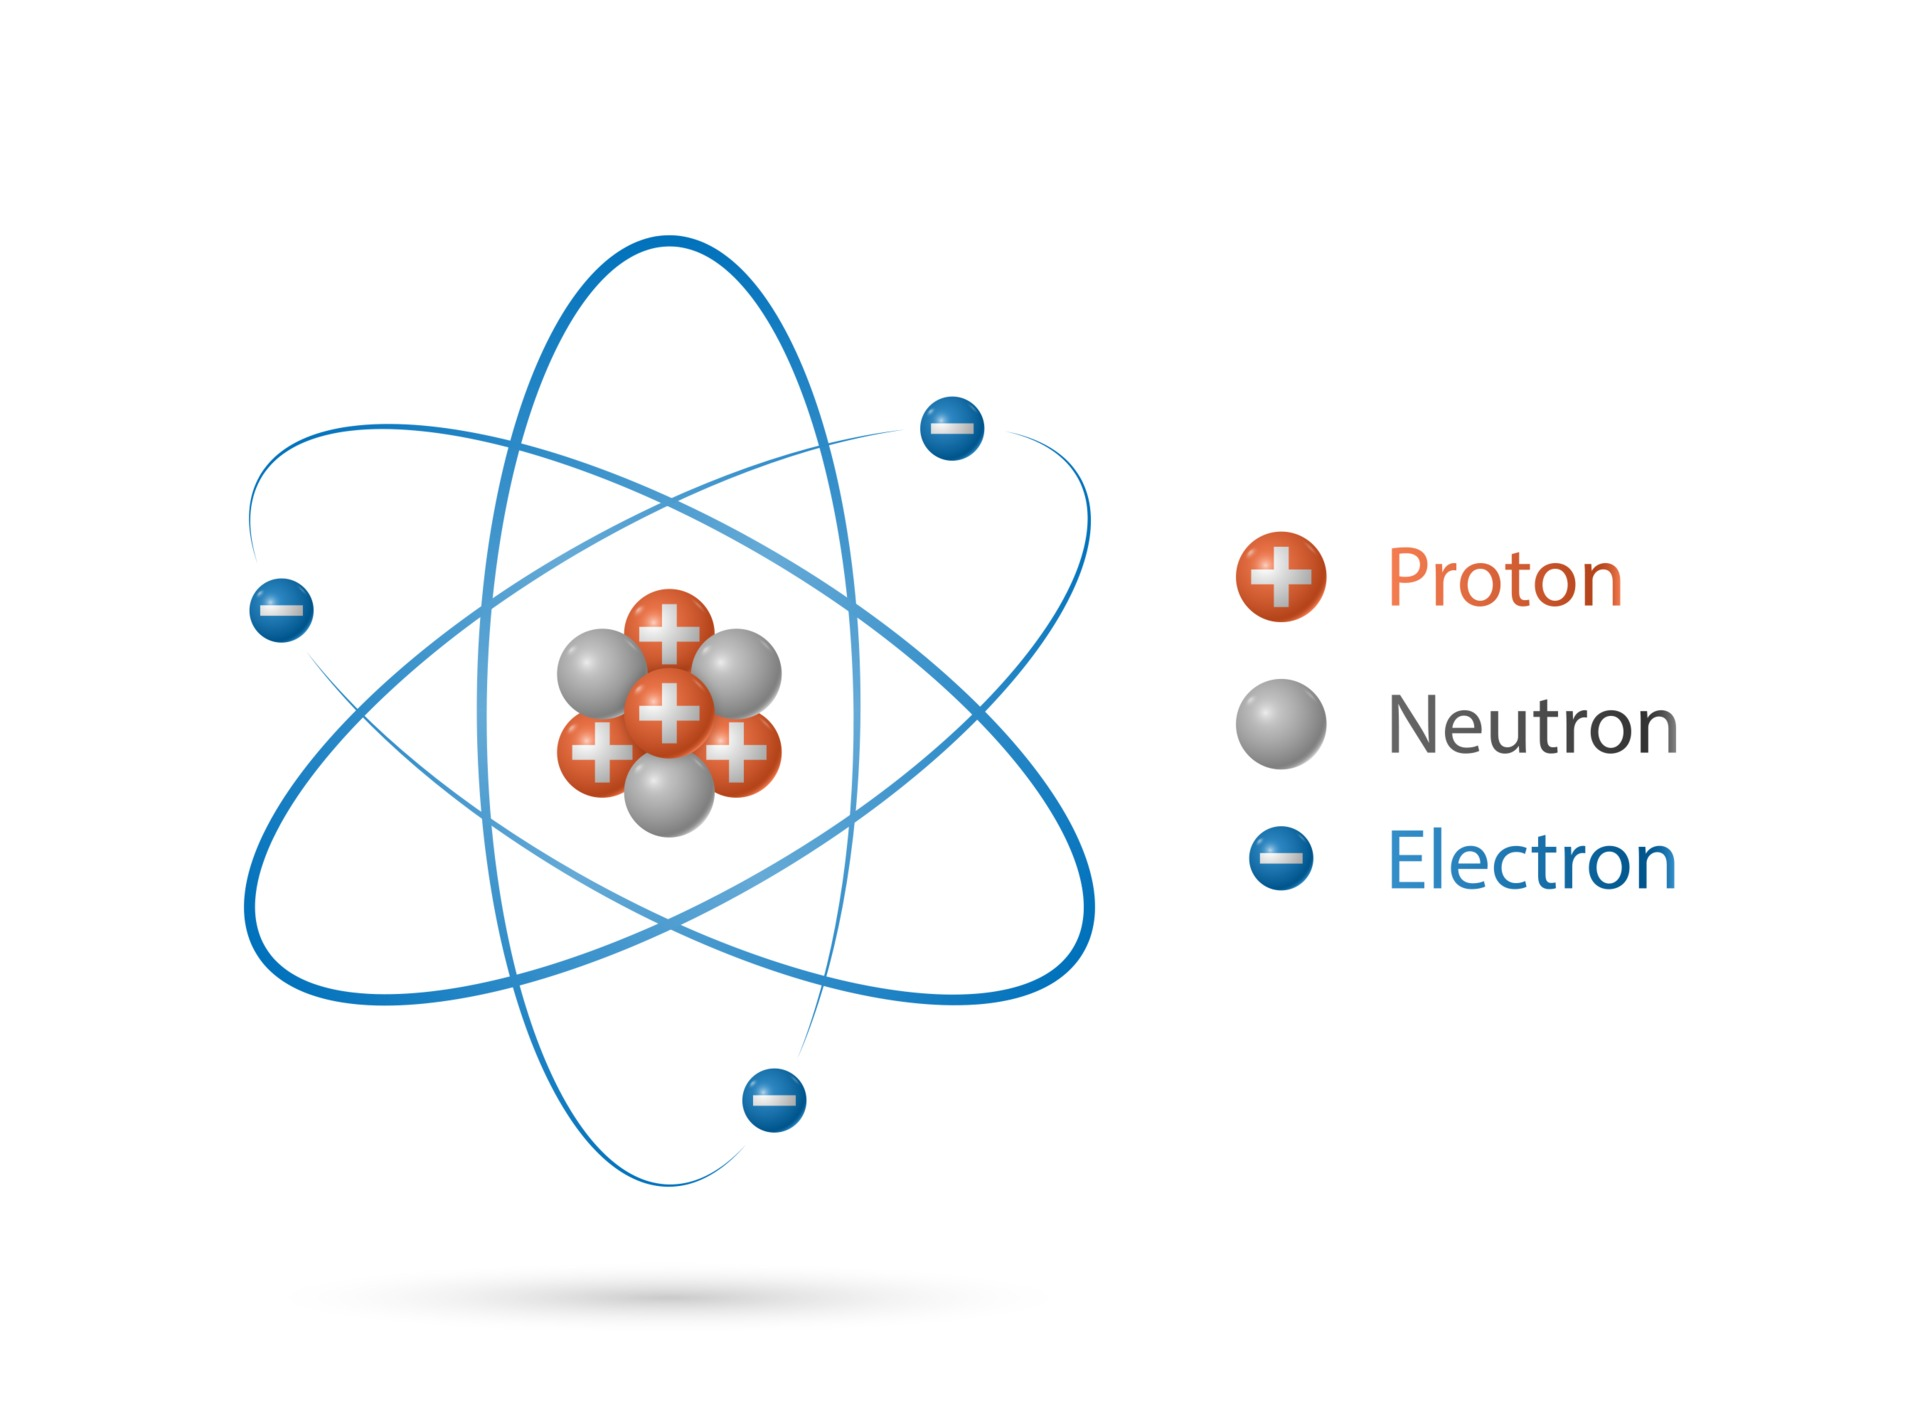
\includegraphics[width=0.4\textwidth]{atom_struct.jpg}
    \caption{Estructura básica de un átomo.}
    \label{fig:atom_struct}
\end{figure}

Esta estructura corresponde a un \textbf{modelo atómico}, que es una representación que nos ayuda a entender cómo está compuesto un átomo y cómo se comporta. A lo largo del tiempo han existido distintos modelos atómicos, pero uno de los más conocidos es el \textbf{modelo de Bohr}. Según este modelo, los electrones giran alrededor del núcleo en \textbf{órbitas circulares}, cada una con un nivel de energía específico. Cuando un electrón cambia de órbita, absorbe o emite energía en forma de luz.

La carga elemental \colorbox{highlight}{\( e \)} es la \textbf{cantidad más pequeña de carga eléctrica libre que se conoce en la naturaleza}. Es la carga que poseen los protones y electrones, pero con signo opuesto:
\begin{itemize}
    \item \textbf{Electrón}: \( -e = -1.602 \times 10^{-19} \) C (coulombs)
    \item \textbf{Protón}: \( +e = 1.602 \times 10^{-19} \) C
\end{itemize}

La carga elemental es fundamental porque todas las cargas eléctricas observadas en la naturaleza son \textbf{múltiplos enteros de \( e \)}. Es decir, cualquier carga presente en un objeto es el resultado de un exceso o déficit de electrones. Este principio se conoce como la \textbf{ley de conservación de la carga eléctrica}, y establece que la carga eléctrica \textbf{no se crea ni se destruye}, solo se transfiere de un cuerpo a otro.  

Los objetos tienen carga debido a la presencia de \textbf{electrones y protones}. Un objeto es eléctricamente neutro cuando tiene igual número de ambos. Si un objeto adquiere carga negativa, significa que ha \textbf{ganado electrones}, y si adquiere carga positiva, significa que ha \textbf{perdido electrones}. Cuando un objeto se carga, no se están creando nuevas cargas, sino que \textbf{se están moviendo electrones} de un cuerpo a otro. Por ejemplo: en la \textbf{electrización por frotamiento}, un material transfiere electrones a otro, dejando uno cargado positivamente y el otro negativamente. En la \textbf{inducción}, un objeto cargado puede redistribuir las cargas en otro sin tocarlo, pero sin cambiar la cantidad total de carga en el sistema.

En otras palabras, la carga eléctrica siempre se conserva porque \textbf{los electrones y protones no se destruyen en procesos normales}, solo cambian de ubicación dentro de un sistema.

\colorbox{highlight}{Denominaremos con la letra \( Q \) o \( q \) a la carga eléctrica de un objeto.} La carga se mide en \textbf{coulombs (C)}. Un coulomb es una cantidad de carga muy grande, por lo que en la práctica se utilizan submúltiplos como el \textbf{millicoulomb (mC)} o el \textbf{microcoulomb (\( \mu \text{C} \))}.

\subsection{Fuerza y campo eléctrico}

\subsubsection{Ley de Coulomb}

La electrostática estudia las cargas eléctricas en \hl{\textbf{reposo}}. La ley de Coulomb establece que \textbf{la fuerza entre dos cargas puntuales} es:

\begin{equation}
    F = k_e \frac{\abs{q_1} \cdot \abs{q_2}}{r^2}
    \label{eq:ley_coulomb}
\end{equation}

donde:

\begin{itemize}
    \item \( k_e \) es la constante de Coulomb: \( 8.9876 \times 10^9 \, \frac{\si{\newton\meter\squared}}{\si{\coulomb\squared}} \).
    \begin{itemize}
        \item \( k_e \) se obtiene de  \( \frac{1}{4\pi\epsilon_0} \) y,
        \item \( \epsilon_0 \) es la permitividad del vacío: \( 8.85 \times 10^{-12} \,\frac{\si{\coulomb\squared}}{\si{\newton\meter\squared}} \)
    \end{itemize}
    \item \( q_1 \) y \( q_2 \) son las cargas.
    \item \( r \) es la distancia entre las cargas.
\end{itemize}

Es muy importante notar que la \textbf{Ley de Coulomb} \eqref{eq:ley_coulomb} se aplica estrictamente a \hl{cargas puntuales}, es decir, cargas que se consideran concentradas en un solo punto sin dimensiones espaciales. En la ecuación anterior \eqref{eq:ley_coulomb}, se obtiene la magnitud de la fuerza eléctrica. La expresión vectorial de la fuerza eléctrica es:

\begin{equation}
    \vec{F}_e = k_e \frac{|q_1 q_2|}{r^2} \hat{r}
    \label{eq:ley_coulomb_vectorial}
\end{equation}

donde:
\begin{itemize}
    \item \( \vec{F}_e \) es el vector fuerza eléctrica entre dos cargas puntuales \( q_1 \) y \( q_2 \)
    \item \( \hat{r} \) es el vector unitario en la dirección que une ambas cargas.
\end{itemize}

Esto es importante tenerlo en cuenta ya que si se quiere saber la fuerza total sobre una carga \( q \) debido a varias cargas, se debe sumar vectorialmente las fuerzas individuales. La fuerza total sobre una carga \( q \) debido a un conjunto de cargas \( Q_i \) es:

\begin{equation}
    \vec{F} = \sum_i k \frac{|q \cdot Q_i|}{r_i^2} \hat{\mathbf{r_i}}
    \label{eq:ley_coulomb_vectorial_suma}
\end{equation}

\subsubsection{Cargas eléctricas}

La \textbf{carga eléctrica} es una propiedad fundamental de la materia que determina la interacción electromagnética entre partículas. Se trata de una magnitud escalar que puede ser de dos tipos: \textbf{positiva} o \textbf{negativa}. Las partículas con carga del mismo signo se repelen, mientras que las de signo opuesto se atraen.

La unidad de carga eléctrica en el \textbf{Sistema Internacional (SI)} es el \textbf{coulomb (\( \si{coulomb} \))}. La carga elemental está representada por la carga del electrón (\( -e = -1.602 \times 10^{-19} \si{coulomb} \)) y la del protón (\( e = +1.602 \times 10^{-19} \si{coulomb} \)).

\begin{center}
    \setlength{\arrayrulewidth}{1pt}  % Grosor de líneas
    \renewcommand{\arraystretch}{1.3} % Espaciado vertical
    \arrayrulecolor{gray} % Color de líneas

    \begin{tabular}{ c c c }
        \hline
        \rowcolor{asparagus!30}
        \textbf{Partícula}  & \textbf{Carga (\si{C})}           & \textbf{Masa (\si{kg})}   \\ \hline
        Electrón (e)        & \(-e = -1.602 \times 10^{-19}\)   & \(9.109 \times 10^{-31}\) \\
        Protón (p)          & \(+e = +1.602 \times 10^{-19}\)   & \(1.672 \times 10^{-27}\) \\
        Neutrón (n)         & \(0\)                             & \(1.675 \times 10^{-27}\) \\ \hline
    \end{tabular}
\end{center}

\subsubsection{Campo eléctrico}

Para entender la definición del campo eléctrico desde el principio, debemos pensar en cómo se conceptualiza la interacción entre cargas eléctricas y en la necesidad de definir una propiedad del espacio que describa esta interacción.

Sabemos que las cargas eléctricas ejercen fuerzas unas sobre otras. Experimentalmente, se observa que cargas del mismo signo se repelen y cargas de signo opuesto se atraen. Esta interacción fue formulada matemáticamente por la Ley de Coulomb \eqref{eq:ley_coulomb_vectorial}, sin embargo, esta ley solo nos dice cómo una carga afecta a otra en particular, \hl{pero no describe una propiedad del espacio en sí}. Aquí es donde se introduce el concepto de \textbf{campo eléctrico}.

\begin{figure}[ht]
    \centering
    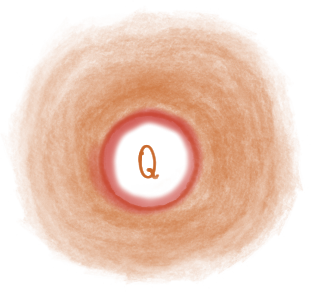
\includegraphics[width=0.4\textwidth]{field_concept.png}
    \caption{Concepto de campo eléctrico.}
    \label{fig:concepto_campo_electrico}
\end{figure}

En lugar de pensar que una carga actúa instantáneamente sobre otra, se puede imaginar que una carga genera algo en el espacio a su alrededor que luego interactúa con otras cargas. Este ``algo'' es el \textbf{campo eléctrico}. La idea es la siguiente:

\begin{enumerate}
    \item Una carga fuente \( Q \) modifica el espacio circundante.
    \item Cualquier otra carga \( q \) que se coloque en ese espacio experimentará una fuerza debido a esta modificación.
    \item Para cuantificar esa modificación, definimos el campo eléctrico como la \textbf{fuerza por unidad de carga de prueba}.
\end{enumerate}

\paragraph{Idea conceptual del campo eléctrico}

Si te preguntas qué es el campo eléctrico, puedes responder según la descripción previa: ``el campo eléctrico es una propiedad del espacio que rodea a una carga eléctrica capaz de interactuar con otras cargas''. Sin embargo la idea es entender qué significa que una carga eléctrica modifique las propiedades del espacio que la rodea. Veamos un ejemplo de esto para entenderlo mejor.

Supongamos que tengo una carga positiva (un protón) y quiero que se quede totalmente quieto. Entonces ¿Cómo podemos lograr esto? 
Bueno, pues es bastante sencillo. Buscamos alguna carga \( Q \) que a una distancia \( r \) haga que la carga \( q \) del protón anule las fuerzas que interactúan con la carga.

Supongamos que la única fuerza que está interactuando con el protón es la fuerza peso. Entonces tendriamos que encontrar cualquier combinación de \( Q \) y \( r \) que cumpla:

\[
    F_g = F_e = k_e \frac{Q \cdot q}{r^2}
\]

Como nuestras incógnitas son \( Q \) y \( r \) vamos a tener infinitas posibilidades que solucionan muestro problema. Pero antes de dar por terminado el problema te pregunto ¿Qué tienen en común todas las soluciones?

Todas las soluciones están ocacionando el mismo efecto en el protón, una fuerza vertical y hacia arriba (en sentido opuesto al peso). Podriamos expresar esto diciendo: ``todas las soluciones generan una perturbación identica en el punto del espacio donde se encuentra el protón''. O, en otras palabras, todas las soluciones generan un campo eléctrico de las mismas características en donde está el protón.

Es más, cualquier partícula que coloquemos en el lugar del protón, con cualquier carga, por ejemplo una partícula con tres veces la carga del protón pero negativa, sentirá una fuerza proporcional a la que sentía el protón. En el caso de este ejemlo sería una fuerza igual a tres veces el peso del protón en el mimo sentido al peso (por ser negativa).

\paragraph{Formulando el Campo Eléctrico}

El campo eléctrico \( \vec{E} \) se define como la fuerza por unidad de carga de prueba \textbf{positiva} en un punto en el espacio. Esto puede expresarse como:

\begin{equation}
    \vec{E} = \frac{F}{q^{+}} = k_e \frac{Q}{r^2}
\end{equation}

donde:
\begin{itemize}
    \item \( Q \) es la carga que genera el campo (puntual).
    \item \( r \) es la distancia entre la carga de prueba y \( Q \).
\end{itemize}

En caso de que exista más de una carga que genera el campo, se aplica \textbf{el principio de superposición} que consiste en sumar todos todos los campos vectorialmente.

\[
\vec{E} = \sum{\vec{E}_i} = k \cdot \sum{\frac{Q_i}{r^2_i}} \hat{r}_i
\]

Sin embargo, en muchos casos, tenemos una distribución continua de carga en vez de una colección de cargas discretas. En esta situación, la carga puede estar distribuida a lo largo de una recta, sobre alguna superficie, por todo un volumen. Siguiendo el concepto de superposición de cargas tendríamos:

\[
\vec{E} = k \lim_{\Delta q_i \to 0} \sum_i{\frac{\Delta q_i}{r_i^2}\hat{r}_i} = k \int \frac{dq}{r^2} \hat{r}
\]

En los casos que debemos calcular el campo de una distribución continua tendremos la \textit{densidad de carga}. Pero ¿Qué es la densidad de carga?

La \textbf{densidad de carga} es una \textit{medida de cuánta carga eléctrica hay distribuida} sobre una determinada región del espacio. Se utiliza cuando las cargas no están concentradas en puntos, sino \textbf{distribuidas} sobre líneas, superficies o volúmenes.

Dependiendo del tipo de distribución, hay tres formas principales:

\subparagraph{1. Densidad lineal de carga:}

Se usa cuando la carga está distribuida a lo largo de una línea (como un alambre).

\[
\lambda = \frac{Q}{l} ~ ~ \rightarrow ~ ~ dq = \lambda dl
\]

\begin{itemize}
    \item \( \lambda \): densidad lineal (C/m)  
    \item \( Q \): pequeña cantidad de carga  
    \item \( l \): pequeña longitud del alambre  
\end{itemize}

\subparagraph{2. Densidad superficial de carga:}

Se usa para cargas sobre una superficie (como una lámina metálica cargada).

\[
\sigma = \frac{Q}{A} ~ ~ \rightarrow ~ ~ dq = \sigma dA
\]

\begin{itemize}
    \item \( \sigma \): densidad superficial (C/m²)  
    \item \( Q \): carga sobre un área pequeña  
    \item \( A \): área considerada  
\end{itemize}

\subparagraph{3. Densidad volumétrica de carga:}

Se usa cuando la carga ocupa un volumen (como una nube de plasma).

\[
\rho = \frac{Q}{V} ~ ~ \rightarrow ~ ~ dq = \rho dV
\]

\begin{itemize}
    \item \( \rho \): densidad volumétrica (C/m³)  
    \item \( Q \): carga dentro de un pequeño volumen  
    \item \( V \): volumen correspondiente  
\end{itemize}


Estas densidades permiten convertir una distribución continua de carga en una integral, y así calcular el campo eléctrico o el potencial.  
Por ejemplo, si conocés \( \lambda(x) \), podés calcular el campo eléctrico de una varilla cargada mediante:

\[
\vec{E} = \frac{1}{4\pi\varepsilon_0} \int \frac{\lambda(x)\, dx}{r^2} \hat{r}
\]

\paragraph{Visualización del campo eléctrico}

Para visualizar el campo eléctrico veamos un ejemplo sencillo. Supongamos que tenemos tres cargas eléctricas de distinto valor ubicadas en tres lugares distintos. Todas estas cargas están fijas en su posición y no pueden moverse (ver figura \ref{fig:campo_electrico_ejemplo_1}). 

\begin{figure}[ht]
    \centering
    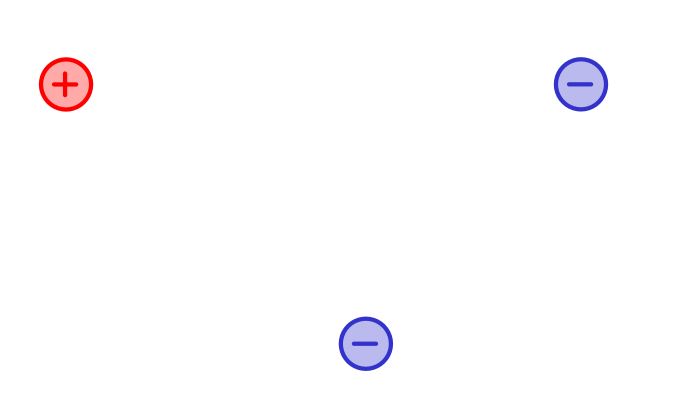
\includegraphics[width=0.5\textwidth]{field_ex_1.png}
    \caption{tres cargas fijas en el espacio.}
    \label{fig:campo_electrico_ejemplo_1}
\end{figure}

Estas tres cargas posicionadas en el espacio constituyen lo que llamaremos \textbf{carga fuente}. Estas tres cargas fuente son capaces de generar una fuerza en cualquier partícula con carga que se coloque en este espacio. Podemos decir entonces, que las tres cargas le dan una propiedad eléctrica al espacio que las rodea. A esta propiedad que adquiere el espacio por culpa de las cargas le llamaremos campo eléctrico y existe independientemente de que haya otra cuarta carga presente o no.

Ahora supongamos que queremos jugar con el campo generado, y tomamos una cuarta carga \( q^{+} \), en este caso la carga será positiva, y la llamaremos \textbf{carga de prueba}. Entonces colocamos la carga de prueba en el centro de las tres cargas y la soltamos (ver figura \ref{fig:campo_electrico_ejemplo_2})

Cuando la soltamos, la carga será empujada hacia algún lugar, ya que, experimentará una fuerza debido a la interacción con las otras cargas. Ya sabemos que las cargas del mismo signo se repelen y las de signo opuesto se atraen.

\begin{figure}[ht]
    \centering
    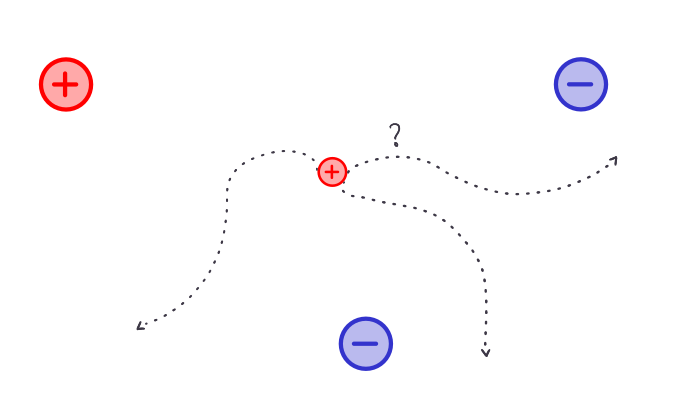
\includegraphics[width=0.5\textwidth]{field_ex_2.png}
    \caption{colocamos una cuarta carga en el centro y la soltamos.}
    \label{fig:campo_electrico_ejemplo_2}
\end{figure}

Entonces aquí tenemos tres cargas aplicando tres fuerzas distintas, ¿qué hacemos? Sumar todas las fuerzas. Algunas se van a contrarrestar un poco al estar en direcciones opuestas, pero otras se van reforzar al tirar en el mismo sentido.

La suma de todas estas fuerzas (fuerza resultante) nos indica hacia dónde va ir la carga y la intensidad del empujón que sentirá (magnitud de la fuerza). Si realizamos esto en cada punto del espacio acabaríamos llenando el espacio de vectores de fuerza, esto se vería como un ``mapa de flechas'' que representan la fuerza que siente la carga de prueba en cada punto.

\textbf{Pero espera:} imaginemos que realizamos todos los cálculos con una carga de prueba de \( 1 \si{\coulomb} \). Y esa carga de prueba en realidad solo la usamos para realizar los cálculos del mapa, pero en realidad no existe. Entonces este mapa lo podemos usar para saber qué fuerza sentiría una carga \( q \) cualquiera.
Seguro te preguntarás ¿Cómo es eso? Es bien sencillo, presta atención a lo siguiente. Si recordamos la ecuación de la fuerza debido a la interacción entre cargas tenemos:

\[
\vec{F}_e = k\frac{Q\cdot q^{+}}{r^2}\hat{r} 
\]

Ahora, recordando que \( Q \) era nuestra carga fuente (formada por las tres cargas) y \( q^{+} \) nuestra carga de prueba de \( 1 \si{\coulomb} \) que usamos para hacer todas las cuentas, si quitamos la carga de prueba, como en la ecuación de fuerza es un factor neutro (multiplica por 1), el resultado no cambiaría cuantitativamente, sin embargo cambiarían las unidades. Veamos como queda:

\[
\vec{F}_e ~ [\si{\newton}] \neq k \frac{Q}{r^2} \hat{r} ~ [\si{\newton\per\coulomb}]
\]

Vemos que lo que resulta es una desigualdad, ya que las unidades no coinciden. Si bien numericamente es lo mismo, dimensionamente no. Para arreglar este problema entonces, en vez de quitar directamente la carga, podemos dividir ambos miembros por \( q^{+} \), y no romperíamos las unidades:

\[
\frac{\vec{F}_e}{q^{+}} ~ [\si{\newton\per\coulomb}] = k \frac{Q}{r^2} \hat{r} ~ [\si{\newton\per\coulomb}]
\]

\begin{figure}[ht]
    \centering
    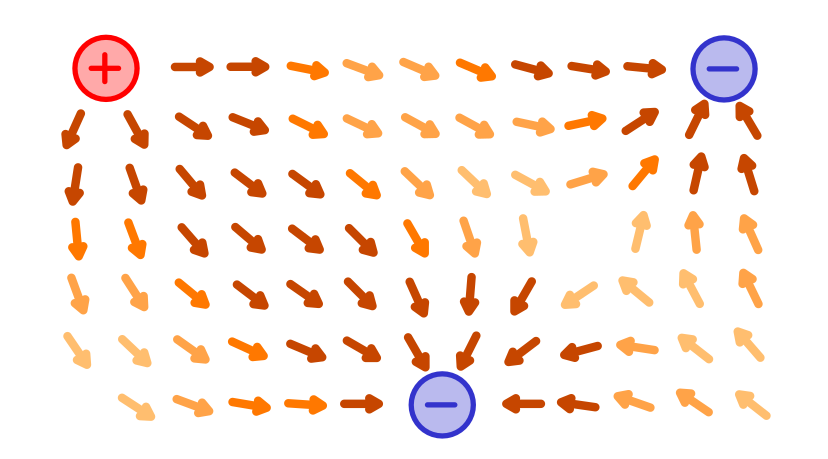
\includegraphics[width=0.5\textwidth]{field_example.png}
    \caption{mapa de la fuerza que siente \(q^{+}\) en cada punto.}
    \label{fig:campo_electrico_ejemplo_3}
\end{figure}

¿Qué nos dice este ``mapa de flechas''? Este mapa de flechas nos dice la \hl{fuerza por unidad de carga} que generan las cargas fuente. Es decir, si colocamos una carga unidad (como \(q^{+}\)), entonces la relación es \(1:1\), pero podemos colocar cualquier carga \(q\) y multiplicarla por el campo.

\begin{equation}
    \vec{E} = \frac{\vec{F}}{q^{+}}
    \label{eq:campo_electrico}
\end{equation}

donde:
\begin{itemize}
    \item \( \vec{E} \) es el campo eléctrico en ese punto,
    \item \( \vec{F} \) es la fuerza experimentada por la carga de prueba \( q^{+} \),
    \item \( q^{+} \) es la carga de prueba.
\end{itemize}

Ahora, como vimos, la carga de prueba es una carga hipotética utilizada para medir el campo sin modificarlo. Como la carga de prueba es positiva, entonces vemos que una carga fuente \(Q\) cualquiera, respeta la siguiente distribución: si la carga \(Q\) es \textbf{negativa}, las líneas de campo son entrantes, si la carga \(Q\) es \textbf{positiva}, las líneas de campo son salientes:

\begin{figure}[ht]
    \centering
    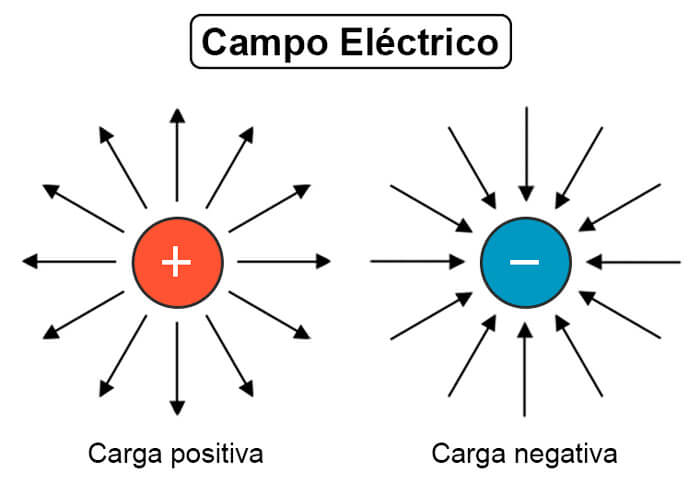
\includegraphics[width=0.5\textwidth]{electric_field.jpg}
    \caption{Campo eléctrico de una carga puntual positiva y una negativa.}
    \label{fig:campo_electrico}
\end{figure}

Este resultado nos dice que el \hl{campo eléctrico} \textbf{se aleja} de cargas positivas y \textbf{se dirige hacia} cargas negativas. Además disminuye con el cuadrado de la distancia y es una propiedad del espacio ya no depende de la carga de prueba \( q \), sino solo de \( Q \).

Es muy importante tener en cuenta las premisas usadas para formular el \textbf{campo eléctrico}:
\begin{itemize}
    \item \textit{La carga fuente modifica el espacio circundante:} El campo eléctrico es una propiedad del espacio y es generado por una carga fuente.
    \item \textit{El campo es independiente de la carga de prueba:} La carga de prueba se usa solo como herramienta de medición.
    \item \textit{El campo es un campo vectorial:} Tiene dirección y magnitud en cada punto del espacio.
    \item \textit{El campo sigue el principio de superposición:} Si hay varias cargas, el campo total en un punto es la suma vectorial de los campos generados por cada una.
    \item \textit{La carga de prueba es positiva:} Para determinar el sentido del campo es importante tener en cuenta que la carga de prueba es positiva, esto permite ver con claridad cuando el campo es entrante o saliente para una carga puntual, o poder predecir correctamente el sentido del campo en una distribución de cargas (ya sea discreta o continua).
\end{itemize}

\subsubsection{Lineas de campo eléctrico}

Las líneas de campo no son más que un medio para visualizar el patrón formado por el campo eléctrico a través del trazo de líneas conocidas como \textbf{líneas de campo eléctrico}. Estas líneas relacionan el campo eléctrico con una región del espacio de la siguiente manera:
\begin{itemize}
    \item El vector \(\vec{E}\) del campo eléctrico es tangente a la línea del campo eléctrico en cada punto y la dirección de la linea de campo es igual a la del campo eléctrico.
    \item El número de líneas de campo que pasan por una superficie perpendicular a dichas líneas es proporcional a la magnitud de campo.
\end{itemize}

\begin{figure}[ht]
    \centering
    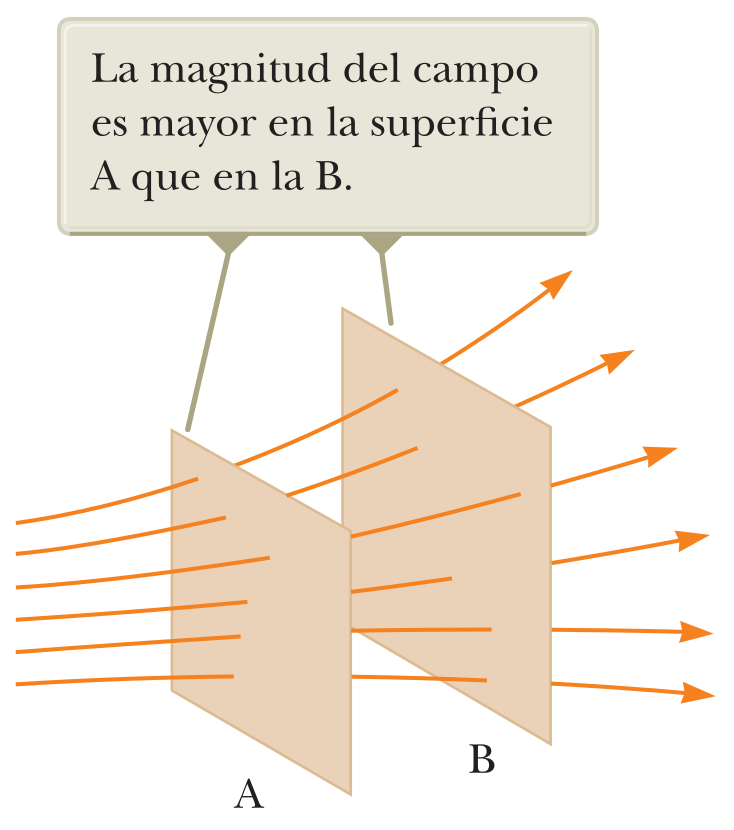
\includegraphics[width=0.5\textwidth]{field-lines.png}
    \caption{Líneas de campo eléctrico que atraviesan dos superficies}
    \label{fig:lineas_de_campo}
\end{figure}

Pongamos este concepto en palabras simples ¿Recuerdas el ejemplo de las tres cargas y el ``mapa de flechas''? Bueno, las líneas de campo nos ayudan a visualizar el ``mapa de flechas'' de una forma más cómoda.

\begin{figure}[ht]
    \centering
    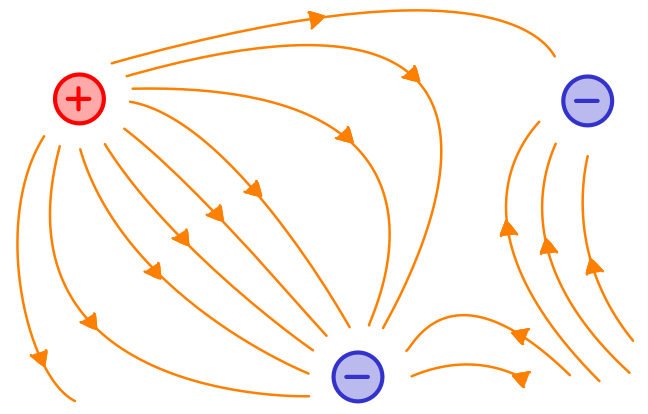
\includegraphics[width=0.4\textwidth]{field_lines_ex.png}
    \caption{Ejemplo del ``mapa de flechas'' visualizado con líneas de campo}
    \label{fig:ej_lineas_de_campo}
\end{figure}

En este caso se puede ver que las líneas de campo están más juntas cuando nos acercamos a las cargas, y se van separando cuando nos alejamos. La proximidad entre líneas de campo nos indica que el campo es intenso. Si las líneas están distantes entre sí indica que el campo es menos intenso. Esto se puede verificar con la ecuación del campo eléctrico, ya que el campo disminuye con el cuadrado de la distancia. Esto significa que según más nos alejamos de las cargas fuente, el campo disminuye.

\subsection{Flujo eléctrico}

\subsection{Flujo eléctrico}
\label{sec:flujo_electrico}

Hasta ahora hemos visto una idea general de las líneas de campo eléctrico. Es decir, vimos una explicación que busca dar una idea general de cómo funcionan las líneas de campo eléctrico, su forma, su dirección y su relación con las cargas, pero sin proporcionar fórmulas o cantidades específicas. En este apartado, vamos a explicar con mayor formalidad este concepto, donde se considerará la magnitud del campo eléctrico y el área a través de la cual se mide el flujo eléctrico, utilizando la relación matemática entre estas variables.

\subsubsection{Definición}

El \hl{flujo eléctrico} es una medida de la cantidad de campo eléctrico que atraviesa una superficie dada. Se define matemáticamente como el producto de la magnitud del campo eléctrico (\(E\)) y el área (\(A\)) de la superficie a través de la cual se mide el flujo, así como el coseno del ángulo (\(\theta\)) entre la dirección del campo eléctrico y la normal (perpendicular) a la superficie. La fórmula para calcular el flujo eléctrico (\(\Phi_E\)) es:

\begin{figure}[ht]
    \centering
    \begin{subfigure}[b]{0.45\textwidth}
        \centering
        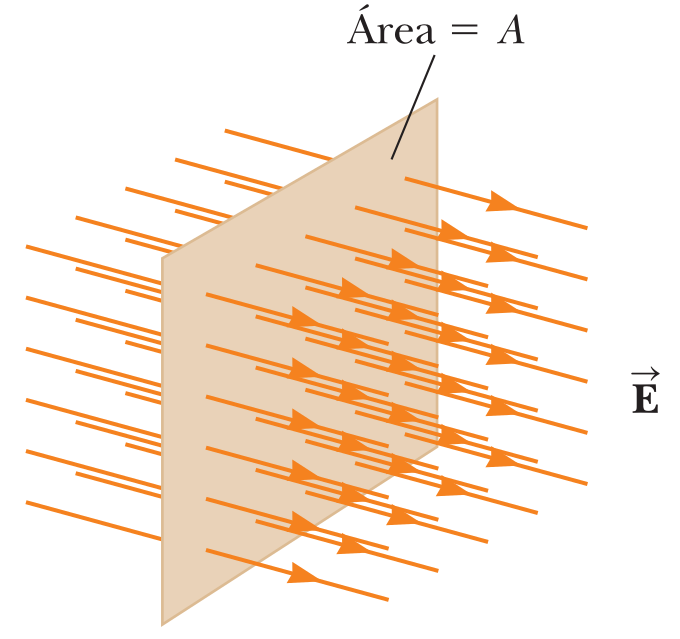
\includegraphics[width=\textwidth]{flujo_1.png}
        \caption{flujo sobre un area perpendicular.}
        \label{fig:flujo1}
    \end{subfigure}
    \hfill
    \begin{subfigure}[b]{0.45\textwidth}
        \centering
        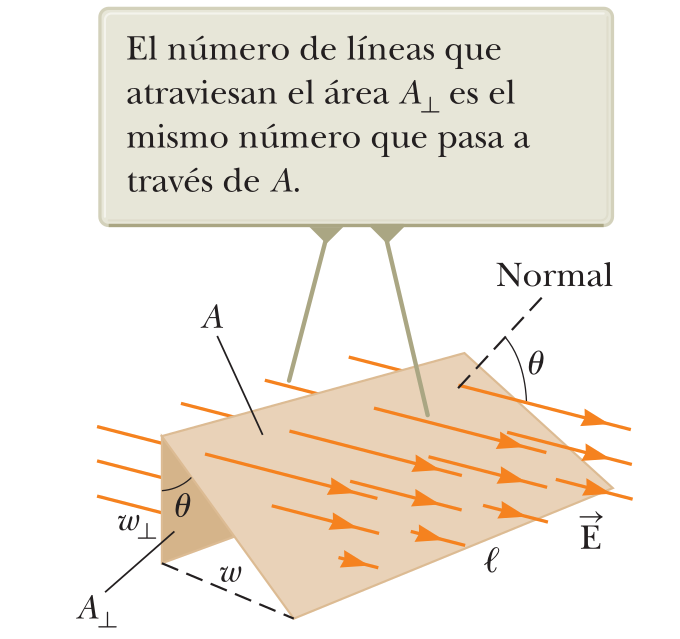
\includegraphics[width=\textwidth]{flujo_2.png}
        \caption{flujo sobre un area inclinada.}
        \label{fig:flujo2}
    \end{subfigure}
    \caption{Flujo eléctrico}
    \label{fig:flujo eléctrico}
\end{figure}

\[
\Phi_E = E \cdot A \cdot \cos(\theta)  ~~ \left[\frac{\si{\newton \meter \squared}}{\si{\coulomb}}\right]
\]

Donde:
\begin{itemize}
    \item \(\Phi_E\) es el flujo eléctrico.
    \item \(E\) es la magnitud del campo eléctrico.
    \item \(A\) es el área de la superficie.
    \item \(\theta\) es el ángulo entre la dirección del campo eléctrico y la normal a la superficie.
\end{itemize}

Otra forma más general de escribir el flujo eléctrico es usando el \hl{producto escalar}. Para poder usar el producto escalar, necesitamos dos vectores, y en este caso solo tenemos el vector de campo. Entonce podemos definir un vector normal a la superficie con igual magnitud al área de la superficie. Entonces el producto escalar entre el vector campo eléctrico (\(\vec{E}\)) y el vector normal al area \(\vec{A}\) es:

\begin{equation}
    \Phi_E = \vec{E} \cdot \vec{A} = E A \cos \theta
    \label{eq:flujo_electrico}
\end{equation}

Hay que tener muy presente que \(\Phi_E\) es un \textbf{ESCALAR} no un vector. Y otro factor a considerar es que la ecuación \eqref{eq:flujo_electrico} solo se puede usar si el campo \(\vec{E}\) es constante. Sin embargo, en general, el campo \(\vec{E}\) no suele ser constante, entonces una forma de conseguir el flujo eléctrico total en una superficie \(S\) donde el campo no es constante es sumando todas las pequeñas contribuciones de flujo eléctrico en pequeñas porciones de area (\(dA\)), resultando en la siguiente integral:

\begin{equation}
    \Phi_E = \int_{S} \vec{E} \cdot d\vec{A}
    \label{eq:flujo_electrico_integral}
\end{equation}

\subsubsection{Ley de Gauss}
\label{sec:ley_de_gauss}

El flujo eléctrico es importante en el estudio del electromagnetismo porque está relacionado con la ley de Gauss, que establece que el flujo eléctrico a través de una superficie \textbf{cerrada} (con frecuencia llamada \textit{superficie gaussiana}) es proporcional a la carga eléctrica total encerrada dentro de esa superficie. Suponga una carga puntual positiva \(q\) ubicada en el centro de una esfera de radio \(r\) como se observa en la figura \ref{fig:superficie_gaussiana}.

\begin{wrapfigure}{r}{0.35\textwidth}
    \centering
    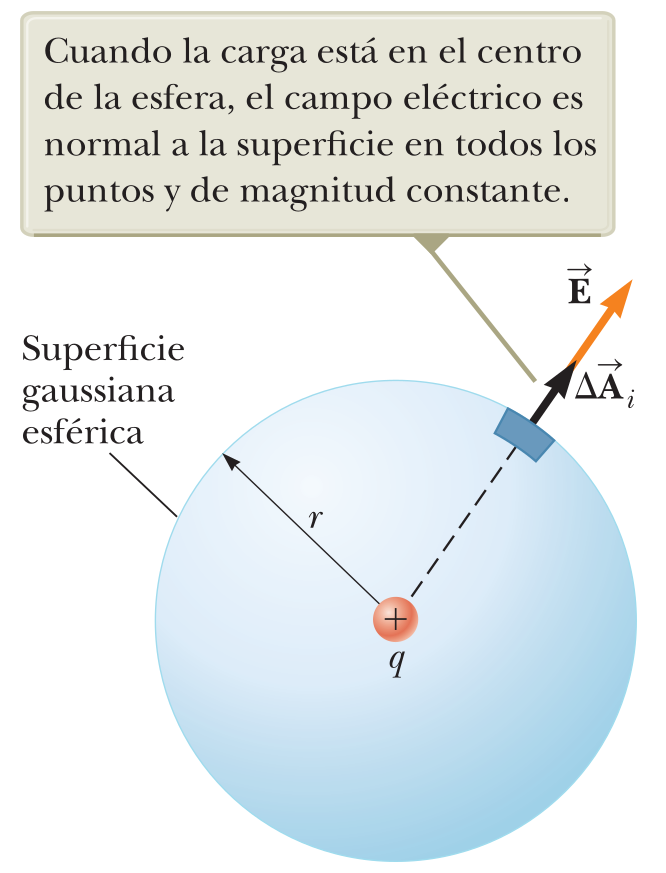
\includegraphics[width=\linewidth]{ley_de_gauss.png}
    \caption{Superficie gaussiana esférica de radio \(r\) que rodea una carga puntual \(q\).}
    \label{fig:superficie_gaussiana}
\end{wrapfigure}
De la ecuación de campo eléctrico \eqref{eq:campo_electrico}, se sabe que la magnitud del campo eléctrico sobre todos los puntos de la superficie (\(S\)) de la esfera es \(\vec{E} = k q/r^2\). Las líneas de campo están dirigidas radialmente hacia afuera y por tanto son perpendiculares a la superficie en todos sus puntos. Es decir, en cada punto de la superficie, \(\vec{E}\) es paralelo al vector \(d\vec{A}\) que representa un elemento de área muy pequeño que rodea al punto en la superficie. Por lo tanto, el flujo neto a través de la superficie gaussiana es igual a:

\begin{align*}
    \Phi_E =& \oint_S \vec{E} \cdot d\vec{A} \\
            =& \oint_S E \cos(0) ~ dA \\
            =& \oint_S E ~ dA \\
    \Phi_E =& E ~ \oint_S dA
\end{align*}
aquí tenemos que \(E=kq/r^2\) donde \(r\) es conocido y vale el radio de la esfera, \(q\) es el valor de la carga en el centro de la esfera y \(k = 1/4\pi\epsilon_0\). Luego la integral resulta en la superficie de una esfera que es \(4\pi r^2\). Entonces:

\[
\Phi_E = E ~ \oint_S dA = \frac{q}{4\pi \epsilon_0 r^2} \cdot 4\pi r^2 = \boxed{\frac{q}{\epsilon_0}} 
\]

Este resultado dice muchas cosas:
\begin{itemize}
    \item \textbf{Primero}: el flujo eléctrico \(\Phi_E\) no depende del radio de la superficie esférica.
    \item \textbf{Segundo}: el flujo es directamente proporcional a la carga encerrada en el interior de la superficie gaussiana.
    \item \textbf{Tercero}: el flujo es inversamente proporcional al valor de \(\epsilon\), en el ejemplo se trabajó con vacío, pero puede ser cualquier material no conductor con otro valor de \(\epsilon\).
\end{itemize}

En base a esto podemos sacar una conclusión, supongamos ahora que la superficie no es esférica ¿El flujo será el mismo que el de la esfera? Bueno, pues voy a hacer un adelanto, si lo es, pero ¿Por qué? Pensemos en la definición de flujo, sea cualquier superficie que rodea la esfera, el flujo será igual a el \(\vec{E}\cdot d\vec{A}\). Como vimos anteriormente esto representa la cantidad de líneas de campo que pasan por una superficie determinada. Como la superficie encierra la misma carga entonces saldrán la misma cantidad de líneas de campo por la superficie.

En este punto tal vez te preguntes ¿Cómo puede ser que no dependa del radio de la esfera, o mejor del tamaño de la superficie arbitraria cerrada? Es sencillo, si el tamaño de la superficie cerrada aumenta, entonces la distancia a la carga encerrada también aumentará, esto significa que la intensidad del campo disminuirá, entonces pasarán menos líneas de campo por cada \(dA\), pero como la superficie total a aumentado, entonces compensará la pérdida de intensidad del campo.

Con esto podemos armar una conclusión:

\begin{tcolorbox}[myconclusion]
    el flujo neto a través de \textit{cualquier} superficie cerrada que rodea a una carga puntual \(q\) está dado por \(q/\epsilon_0\) y es independiente de la forma de la superficie.
\end{tcolorbox}

Entonces, si suponemos varias superficies, llamemos \(S1\), \(S2\) y \(S3\) a las superficies que rodean la carga \(q\) (ver figura \ref{fig:superficie_gaussiana_arbitraria}). Todas estas superficies tienen el mismo flujo eléctrico, ya que todas encierran la misma carga \(q\). Se puede ver que el flujo neto es el mismo para todas las superficies.

\begin{figure}[ht]
    \centering
    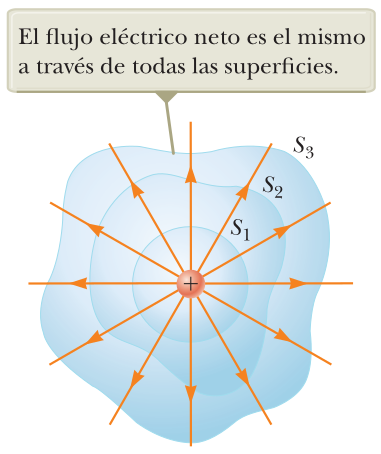
\includegraphics[width=0.35\textwidth]{flujo_neto.png}
    \caption{Distintas superficies gaussianas de forma arbitraria que rodean una carga puntual \(q\).}
    \label{fig:superficie_gaussiana_arbitraria}
\end{figure}

Por otro lado, si la carga \(q\) está fuera de la superficie gaussiana entonces la misma cantidad de líneas de campo que entran por un lado de la superficie, salen por el otro lado. Por lo tanto, el flujo neto a través de la superficie es cero. Esto se puede ver en la figura \ref{fig:flujo_neto_2} donde se observa que el flujo neto es cero.

\begin{figure}[ht]
    \centering
    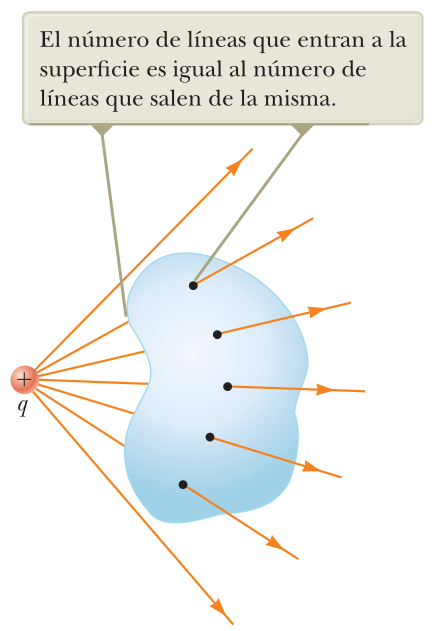
\includegraphics[width=0.4\textwidth]{flujo_neto_externo.png}
    \caption{Una carga puntual \(q\) fuera de la superficie.}
    \label{fig:flujo_neto_2}
\end{figure}

La forma matemática de ley de Gauss, es una generalización de lo anterior y establece que el flujo neto a través de cualquier superficie cerrada es

\begin{equation}
    \Phi_E = \oint_{S} \vec{E} \cdot d\vec{A} = \frac{q_{\text{int}}}{\varepsilon_0} ~~ \left[\frac{\si{\newton \meter \squared}}{\si{\coulomb}}\right]
\end{equation}
donde:
\begin{itemize}
    \item \( \Phi_E \) es el flujo de campo eléctrico a través de una superficie cerrada.
    \item \(E\) es el campo eléctrico en cada punto de esa superficie.
    \item \(dA\) es un vector diferencial de área que apunta hacia afuera de la superficie.
    \item \(q_{int}\) es la carga total encerrada dentro de la superficie.
    \item \(\epsilon_0\) es la permitividad del vacío, una constante del medio.
\end{itemize}

\begin{tcolorbox}[mydanger]
    CUIDADO: \(\vec{E}\) representa el campo eléctrico total, que incluye contribuciones de ambas cargas tanto del interior como del exterior de la superficie.    
\end{tcolorbox}

\paragraph{¿Qué nos dice esta ley, en términos simples?}

El flujo eléctrico representa la cantidad de ``líneas de campo eléctrico'' que atraviesan una superficie. La ley de Gauss nos habla de superficies cerradas, y nos dice que si hay carga dentro de una superficie cerrada, el campo eléctrico ``sale'' (o ``entra'') por esa superficie, generando un flujo distinto de cero. Si no hay carga neta dentro, el flujo eléctrico total es cero, aunque el campo pueda no ser nulo en todos los puntos. No importa la forma de la superficie, solo importa cuánta carga encierra, no cómo se distribuye el campo en detalle.

\subparagraph{¿Por qué es útil la ley de Gauss?}

La ley de Gauss es útil porque, en situaciones con alta simetría (esférica, cilíndrica, planar), permite calcular el campo eléctrico sin integrar la ley de Coulomb, por ejemplo:
\begin{itemize}
    \item Una esfera cargada uniformemente
    \item Un hilo infinitamente largo con carga lineal uniforme
    \item Un plano infinito cargado
\end{itemize}

\subparagraph{Ejemplo clásico: esfera cargada}

Supón una carga distribuida uniformemente en una esfera. Si elegimos una superficie esférica de radio  mayor al de la esfera, por simetría:
\[
\vec{E} = \text{constante} \quad \text{y} \quad \vec{E} \parallel d\vec{A}
\]
Entonces la integral se simplifica:
\[
\oint \vec{E} \cdot d\vec{A} = E \oint dA = E(4\pi r^2)
\]
Y por la ley de Gauss:
\[
E(4\pi r^2) = \frac{Q}{\varepsilon_0} \quad \Rightarrow \quad E = \frac{1}{4\pi\varepsilon_0} \frac{Q}{r^2}
\]
¡Y así recuperamos la fórmula del campo eléctrico de una carga puntual!

\subsection{Potencial eléctrico}

\subsection{Potencial eléctrico}

Cuando se coloca una carga \(q\) en un campo eléctrico \(\vec{E}\), la carga experimenta una fuerza \(\vec{F}=q\vec{E}\). Esta fuerza es conservativa, lo que significa que el trabajo realizado por la fuerza al mover la carga entre dos puntos \(A\) y \(B\) no depende de la trayectoria seguida, sino solo de los puntos inicial y final.

El trabajo realizado por la fuerza al mover la carga \(q\) desde el punto \(A\) hasta el punto \(B\) se define como:
\begin{equation*}
    W_{AB} = \int_A^B \vec{F} \cdot d\vec{s} = \int_A^B q\vec{E} \cdot d\vec{s}
\end{equation*}
donde \(d\vec{s}\) es un elemento diferencial de desplazamiento a lo largo de la trayectoria. Y como la fuerza eléctrica es conservativa, podemos expresarla en términos de la energía potencial eléctrica \(U\):
\begin{equation*}
    W_{AB} = U_A - U_B = -\Delta U
\end{equation*}

\subsubsection{Definición de potencial eléctrico}

Para una posición conocida de la carga de prueba en el campo, el sistema carga-campo tiene una energía potencial \(U\) relativa a la configuración del sistema definida como \(U=0\). Al dividir la energía potencial entre la carga de prueba \(q\), obtenemos el \textbf{potencial eléctrico} \(V\) en un punto \(P\) del campo eléctrico:

\begin{equation}
    V = \frac{U}{q}
    \label{eq:potential}
\end{equation}

El potencial eléctrico es una magnitud escalar que se mide en \(\text{V}\) (voltios) y se define como la energía potencial por unidad de carga.

Teniendo en cuenta la definición de potencial (ecuación \eqref{eq:potential}) la \textbf{diferencia de potencial} \(\Delta V = V_B - V_A\) entre dos puntos \(A\) y \(B\) en un campo eléctrico se define como el cambio en energía potencial por unidad de carga al mover una carga de prueba \(q\) entre esos dos puntos:

\begin{equation}
    \Delta V = \frac{\Delta U}{q} = -\int_A^B \vec{E} \cdot d\vec{s}
    \label{eq:potential_difference}
\end{equation}

Por la ecuación \eqref{eq:potential_difference}, el trabajo realizado por un agente externo al desplazar una carga \(q\) a través de un campo eléctrico con una velocidad constante es:

\[
W=q\Delta V
\]

Es muy importante que el desplazamiento de la carga \(q\) sea a velocidad constante, ya que si no lo es, el trabajo realizado por el agente externo no será igual al trabajo realizado por la fuerza eléctrica. 

Nótese que el concepto de potencial eléctrico se concive de forma similar al de campo eléctrico. Se usa una carga de prueba positiva \(q\) haciendo que sólo dependa de la carga fuente \(Q\) que genera el campo eléctrico. 

\subsubsection{Diferencia de potencial en un campo eléctrico uniforme}

La ecuación \eqref{eq:potential_difference} es válida en todos los campos eléctricos, sean uniformes o no. En un campo eléctrico uniforme, la magnitud del campo \(\vec{E}\) es constante y la dirección de \(\vec{E}\) es la misma en todos los puntos del campo. En este caso, la diferencia de potencial entre dos puntos \(A\) y \(B\) separados por una distancia \(d\) en la dirección del campo eléctrico se puede expresar como:
\begin{equation}
    \Delta V = -\int_A^B \vec{E} \cdot d\vec{s} = -E \, \int_A^B ds = \boxed{-Ed}
    \label{eq:potential_uniform}
\end{equation}
donde \(E\) es la magnitud del campo eléctrico y \(d\) es la distancia entre los puntos \(A\) y \(B\) en la dirección del campo.

El signo negativo indica que el potencial en el punto \(B\) es menor que el potencial en el punto \(A\) si la carga de prueba se mueve en la dirección del campo eléctrico. Esto significa que el trabajo realizado por la fuerza eléctrica es negativo, lo que implica que la energía potencial disminuye al mover la carga en la dirección del campo eléctrico.

\begin{figure}[ht]
    \centering
    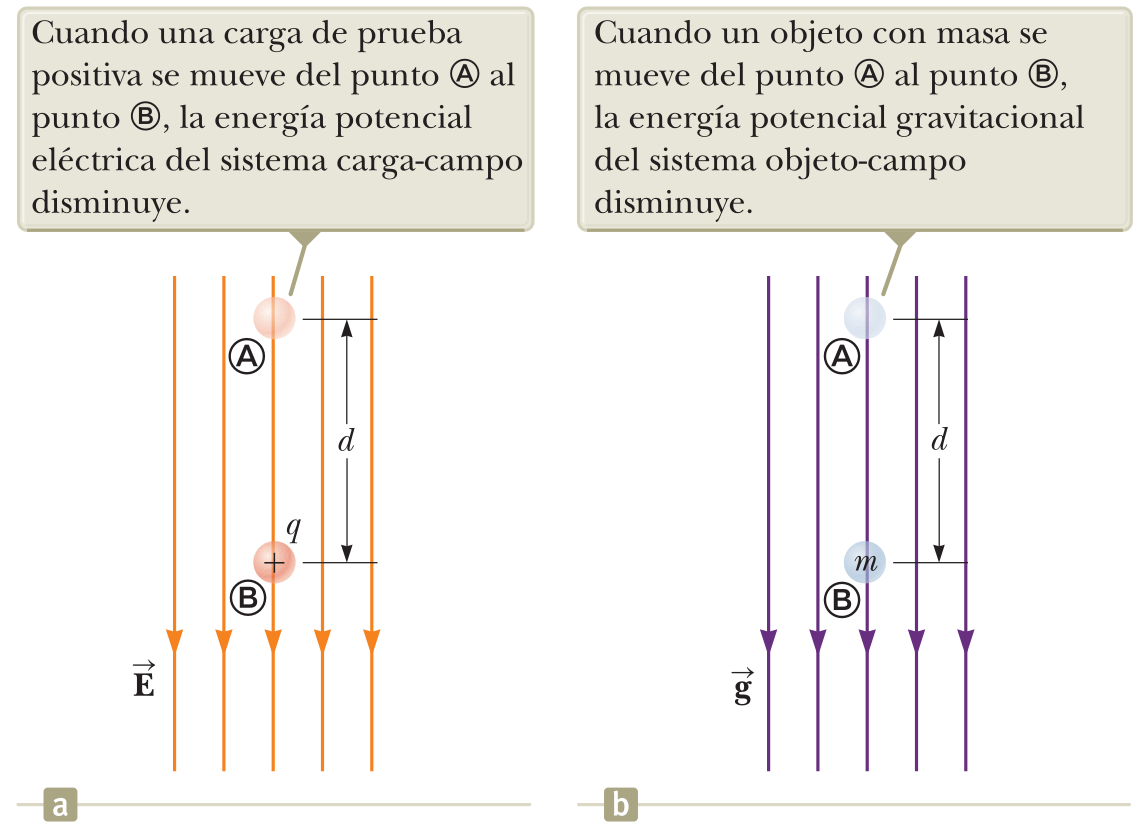
\includegraphics[width=1\textwidth]{potential_const_field.png}
    \caption{Comparación de la energía potencial eléctrica y gravitatoria.}
    \label{fig:potential_uniform}
\end{figure}

\begin{tcolorbox}[mydanger]
    CUIDADO: si la carga \(q\) es negativa, la situación se invierte. El sistema gana energía potencial al mover la carga \(q\) en la dirección del campo eléctrico, y disminuye al moverla en la dirección opuesta.    
\end{tcolorbox}

\subsubsection{Potencial eléctrico debido a una carga puntual}

\begin{wrapfigure}{l}{0.32\textwidth}
    \centering
    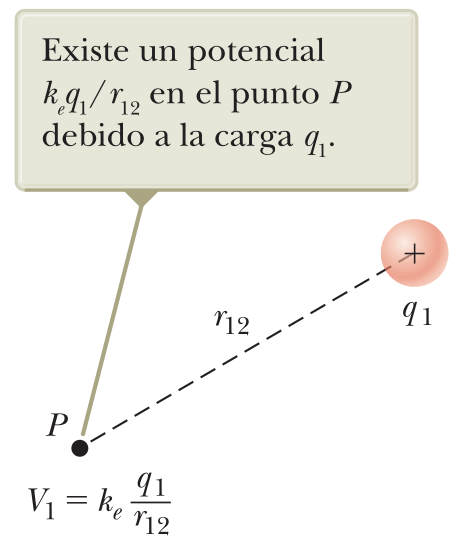
\includegraphics[width=\linewidth]{puntual_potential_1.png}
    \caption{Potencial en el punto \(P\) debido a \(q_1\).}
    \label{fig:potential_point_charge}
\end{wrapfigure}

Como se menciona en la definición, la energía potencial es relativa al punto que se ha definido como ``0''. Con  el potencial eléctrico pasa lo mismo, entonces si queremos saber el potencial en un punto \(P\) del campo eléctrico, sabemos que es igual al trabajo realizado por la fuerza eléctrica al mover una carga de prueba \(q\), pero ¿Desde donde hasta donde? Bueno, podemos definir que nuestro potencial sea cero cuando la carga \(q\) esté infinitamente alejada de la fuente. Entonces el potencial en el punto \(P\) es trabajo para mover la carga de prueba desde el infinito hasta el punto \(P\):

\begin{align*}
    V_P &= - \lim_{a \to \infty}\int_{a}^P \vec{E} \cdot d\vec{r}\\
        &= - \lim_{a \to \infty}\int_{a}^P \frac{kq_1}{r^2} \cdot dr\\
        &= -kq_1 \, \lim_{a \to \infty} \int_{a}^P \frac{1}{r^2} \cdot dr\\
        &= -kq_1 \, \lim_{a \to \infty} \left[ -\frac{1}{r} \right]_{a}^P\\
        &= -kq_1 \, \lim_{a \to \infty} \left[ -\frac{1}{P} + \frac{1}{a} \right]\\
        &= -kq_1 \, \left[ -\frac{1}{P} + 0 \right] \\
    V_P &= k\frac{q_1}{r_{12}} = \lVert\vec{E}\rVert \, \lVert\vec{r}_{12}\rVert \cos(0)
\end{align*}
por ser \(\vec{E}\) y \(\vec{r}_{12}\) paralelos. Entonces el potencial eléctrico en un punto \(P\) debido a una carga puntual \(q_1\) es:
\begin{equation}
    \boxed{V_P = k\frac{q_1}{r_{12}} = E \, r_{12}}
    \label{eq:potential_point_charge}
\end{equation}
donde \(q_1\) es la carga fuente, \(E\) el campo generado por \(q_1\) y \(r_{12}\) la distancia a un punto en el campo eléctrico.

El potencial eléctrico debido a múltiples cargas puntuales se basa en el principio de superposición, que establece que el potencial eléctrico total en un punto es igual a la suma algebraica de los potenciales individuales producidos por cada carga.

\begin{equation}
    V_{total} = \sum_{i=1}^{n} V_i = k \sum_{i=1}^{n} \frac{q_i}{r_i}
\end{equation}

\subsubsection{Obtención de \texorpdfstring{\(\vec{E}\)}{E} a partir de \texorpdfstring{\(V\)}{V}}

El campo eléctrico \(\vec{E}\) y el potencial eléctrico \(V\) están relacionados, como se muestra en la ecuación \eqref{eq:potential_point_charge}, que se usa para encontrar \(V\) en un punto cuando se conoce \(\vec{E}\). Sin embargo, también podemos encontrar \(\vec{E}\) a partir de \(V\) usando la relación:

\begin{equation}
    dV = -\vec{E} \cdot d\vec{s}
    \label{eq:field_from_potential_differential}
\end{equation}
y si estamos trabajando con una única coordenada podemos escribir la ecuación \eqref{eq:field_from_potential_differential} como:

\[
    dV = -E \, ds \quad \Rightarrow \quad E = -\frac{dV}{ds}
\]

Sin embargo, en general, el potencial eléctrico es una función de las tres coordenadas espaciales. Si \(V(r)\) se da en coordenadas cartesianas, las componentes \((E_x, E_y, E_z)\) del campo eléctrico pueden ser determinadas fácilmente a partir de \(V(x, y, z)\) como derivadas parciales

\begin{equation}
    \vec{E} = -\nabla V
    \label{eq:field_from_potential}
\end{equation}
donde \(\nabla\) es el operador nabla, que representa el \hl{gradiente del potencial eléctrico}. Esta relación indica que el campo eléctrico es igual al negativo del gradiente del potencial eléctrico. En otras palabras, el campo eléctrico apunta en la dirección de mayor disminución del potencial eléctrico.

\paragraph{Recordatorio: operador nabla}

El operador \textbf{nabla} (\(\nabla\)), también conocido como \textbf{operador del gradiente}, es una herramienta matemática usada en cálculo vectorial y análisis multivariable. Se utiliza para representar derivadas en múltiples dimensiones.

Formalmente, el operador nabla se define como:

\[
\nabla = \left( \frac{\partial}{\partial x}, \frac{\partial}{\partial y}, \frac{\partial}{\partial z} \right)
\]

Es un operador vectorial que, aplicado a diferentes tipos de funciones, da lugar a distintos conceptos. En nuestro caso solo vamos a repasar el concepto de gradiente.

Cuando se aplica el operador nabla a una función escalar \( f(x, y, z) \), produce un \textbf{campo vectorial} que apunta en la dirección de mayor incremento de la función. Se expresa como:

\[
\nabla f = \left( \frac{\partial f}{\partial x}, \frac{\partial f}{\partial y}, \frac{\partial f}{\partial z} \right)
\]

Este vector resultante indica la dirección en la que la función crece más rápidamente y su magnitud corresponde a la tasa de cambio máxima. En el caso de \(\vec{E}\) y \(V\), \(\vec{E}\) es el gradiente de \(V\) representa una función vectorial que apunta en la dirección de mayor aumento del potencial eléctrico.

\subsection{Capacitores}

Un \textbf{capacitor}, también conocido como \textbf{condensador}, es un componente eléctrico pasivo que tiene la capacidad de \textbf{almacenar energía en forma de un campo eléctrico}. Está compuesto por dos conductores (llamados placas) separados por un material dieléctrico, que actúa como aislante.

Cuando se aplica una diferencia de potencial (voltaje) entre las placas, una de ellas acumula carga positiva y la otra carga negativa, generando así un campo eléctrico entre ellas. La capacidad del capacitor para almacenar carga depende de sus características físicas y del dieléctrico utilizado.

La \textbf{capacitancia} es una medida de esa capacidad de almacenamiento de carga eléctrica. Se define como:

\begin{equation}
    C = \frac{Q}{V}
    \label{eq:capacitance}    
\end{equation}

donde:

\begin{itemize}
    \item \( C \) es la \textbf{capacitancia} del capacitor, medida en faradios (\(\si{\farad}\)).
    \item \( Q \) es la \textbf{carga eléctrica} almacenada en el capacitor, medida en coulombs (\(\si{\coulomb}\)).
    \item \( V \) es la \textbf{diferencia de potencial} entre las placas del capacitor, medida en voltios (\(\si{\volt}\)).
\end{itemize}

Un faradio es una unidad muy grande, por lo que en la práctica suelen utilizarse submúltiplos como el microfaradio (\(\mu\si{farad}\)), nanofaradio (n\(\si{\farad}\)) o picofaradio (p\(\si{\farad}\)).

La capacitancia depende de factores. Si se tienen placas paralelas de depende de factores como el área de las placas (\(A\)), la distancia entre ellas (\(d\)) y la permitividad del dieléctrico (\( \varepsilon \)) según la siguiente fórmula:

\[
C = \varepsilon \frac{A}{d}
\]

Este comportamiento hace que los capacitores sean ampliamente utilizados en circuitos electrónicos para funciones como almacenamiento de energía, filtrado, acoplamiento y desacoplamiento de señales, entre otras.

\subsubsection{Geometría de los conductores}

Cuando la \hl{geometría de los conductores} es distinta a la de un capacitor de placas planas y paralelas, la expresión de la capacitancia cambia, aunque el principio físico fundamental sigue siendo el mismo: almacenar energía en forma de campo eléctrico entre conductores separados por un dieléctrico.

En general, la \hl{capacitancia depende de la geometría de los conductores y del medio dieléctrico entre ellos}. A continuación, se presentan algunos casos comunes:

\paragraph{1. Capacitor esférico}

Consiste en dos esferas concéntricas de radios \( R_1 \) (interna) y \( R_2 \) (externa). Su capacitancia es:

\[
C = 4\pi \varepsilon_0 \varepsilon_r \frac{R_1 R_2}{R_2 - R_1}
\]

\paragraph{2. Capacitor cilíndrico}

Está formado por dos cilindros coaxiales, uno de radio interno \( a \) y otro de radio externo \( b \), y de longitud \( L \) (suponiendo \( L \gg b \)). La capacitancia es:

\[
C = \frac{2\pi \varepsilon_0 \varepsilon_r L}{\ln(b/a)}
\]

\paragraph{3. Geometrías irregulares o generales}

En geometrías más complejas, la capacitancia no puede obtenerse de forma analítica sencilla. En estos casos se recurre a:

\begin{itemize}
    \item Métodos numéricos
    \item Aproximaciones analíticas
    \item Medición experimental
\end{itemize}

Cuando se cambia la geometría, ya no es válida la fórmula simple \( C = \varepsilon \frac{A}{d} \). Es necesario **considerar la distribución del campo eléctrico** que surge de la nueva disposición geométrica, y calcular la capacitancia a partir de las definiciones fundamentales, como:

\[
C = \frac{Q}{V}
\]

donde \( V \) ahora debe calcularse usando la ley de Gauss o integrando el campo eléctrico apropiado para la geometría dada.

\subsection{Resumen}
\begin{table}[h]
    \centering
    \renewcommand{\arraystretch}{1.5}
    \begin{tabular}{|>{\bfseries}l|l|}
        \hline
        \textbf{Concepto} & \textbf{Definición Matemática y Explicación} \\ \hline
        
        \textbf{Ley de Coulomb} & 
        $\vec{F} = k \frac{q_1 q_2}{r^2} \hat{r}$ \\
        & Fuerza entre dos cargas puntuales ($q_1$, $q_2$): \\
        & - $k = \frac{1}{4\pi\varepsilon_0}$ (Constante de Coulomb) \\
        & - $r$: Distancia entre cargas, $\hat{r}$: Vector unitario radial. \\ \hline
        
        \textbf{Campo Eléctrico} & 
        $\vec{E} = \frac{\vec{F}}{q_0} = k \frac{Q}{r^2} \hat{r}$ \\
        & Fuerza por unidad de carga ($q_0$) en un punto: \\
        & - Dirección: Radial para cargas puntuales. \\ \hline
        
        \textbf{Flujo Eléctrico} & 
        $\Phi_E = \int_S \vec{E} \cdot d\vec{A}$ \\
        & Medida del "número de líneas de campo" que atraviesan \\
        & una superficie $S$: \\
        & - $d\vec{A}$: Vector área (normal a la superficie). \\ \hline
        
        \textbf{Ley de Gauss} & 
        $\oint \vec{E} \cdot d\vec{A} = \frac{Q_{\text{int}}}{\varepsilon_0}$ \\
        & Relación entre flujo eléctrico a través de una superficie \\
        & cerrada y la carga encerrada ($Q_{\text{int}}$). \\ \hline
        
        \textbf{Energía Potencial} & 
        $U = k \frac{q_1 q_2}{r}$ \\
        & Trabajo para reunir cargas desde el infinito: \\
        & - $U > 0$ (repulsión), $U < 0$ (atracción). \\ \hline
        
        \textbf{Trabajo Eléctrico} & 
        $W = -\Delta U = q \Delta V$ \\
        & Trabajo realizado por el campo para mover una carga $q$: \\
        & - Depende de la diferencia de potencial ($\Delta V$). \\ \hline
        
        \textbf{Potencial Eléctrico} & 
        $V = \frac{U}{q_0} = k \frac{Q}{r}$ \\
        & Energía potencial por unidad de carga ($q_0$): \\
        & - Escalar, medido en voltios (V). \\ \hline
    \end{tabular}
    \caption{Resumen de conceptos fundamentales de Electroestática.}
    \label{tab:electrostatica}
\end{table}
